\documentclass{csse4400}

\usepackage{languages}
\usepackage{fancyhdr}

% RUBRIC
\usepackage{multirow}
\usepackage{array}
\usepackage{xltabular}
\usepackage{pdflscape}
\usepackage{enumitem}
\usepackage{xcolor}

\newcolumntype{P}[1]{>{\centering\arraybackslash}p{#1}}
% RUBRIC

\title{SpamOverflow}
\author{Evan Hughes, Brae Webb and Richard Thomas}
\date{Semester 1, 2024}

\begin{document}

% Custom footer with UQ copyright notice to facilitate takedown requests at academic file sharing sites (e.g. Course Hero or Chegg).
% Requires document to \usepackage{fancyhdr}.

\pagestyle{fancy}

% Remove all default header content.
\fancyhead{} % Clear default header fields.
\renewcommand{\headrulewidth}{0pt} % Remove horizontal rule from header.

% Set footer details.
\setlength{\footskip}{15mm}
\fancyfoot{}  % Clear default footer fields.
\fancyfoot[L]{\small \copyright \ The University of Queensland \the\year\ }
\fancyfoot[R]{\small Page \thepage}

\maketitle

%\warning{This document is a draft and is subject to change.}

\section*{Summary}
In this assignment, you will demonstrate your ability to \textsl{design},
\textsl{implement}, and \textsl{deploy} a web API that can process a high load,
i.e. a scalable application.
You are to deloy an API for scanning and filtering spam/malicious emails.
Specially your application needs to support:
\begin{itemize}
    \item Scanning an email via an API request.
    \item Providing access to a specified REST API, e.g. for use by front-end interfaces and internal teams.
    \item Remaining responsive while scanning emails.
\end{itemize}

\noindent
Your service will be deployed to AWS and will undergo automated correctness and load-testing to ensure it meets the requirements.

\section{Introduction}

%\paragraph{Task}
For this assignment, you are working for SpamOverflow, a new competitor in the email security space. SpamOverflow uses a microservices based architecture to implement their new malicious email filtering platform. The CEO saw on your resume that you are taking Software Architecture and has assigned you to design and implement a service. This service must be scalable to cope with the anticipated large influx of emails.

\paragraph{Requirements}
Email filtering software can filter email as it arrives or after.
SpamOverflow will implement a service that does not impede the flow of traffic (i.e. does not prevent the email arriving).
It will receive an API call when the mail server receives an email message.
The service then pulls the email from the user's inbox as fast as it can to prevent the user from seeing the malicious email or clicking any links.

Commercial email providers send an API request for each email received.
For optimal performance this service needs to be able to handle a large number of requests in a short period of time, so as to not miss any emails.

Since these emails can be dangerous, the service must be able to report that it is bad or good in a timely manner.
Though genuine emails that are incorrectly marked as dangerous should be returned to the user as quickly as possible.

Persistence is an important characteristic of the platform.
Customers will want to analyse why emails were flagged after the fact.
Upon receiving an email scan request, and after filtering, the system must guarantee that the data has been saved to persistent storage before returning a success response.

\section{Interface}
As you are operating in a microservices context, other service providers have been given an API specification for your service.
They have been developing their services based on this specification so you must match it \emph{exactly}.

The interface specification is available to all service owners online: 

\url{https://csse6400.uqcloud.net/assessment/spamoverflow}

\section{Implementation}
The following constraints apply to the implementation of your assignment solution.

\subsection{SpamHammer}

% Change to be only Dr. Richardson's tool and similarity.

You have been provided with a command line tool called \texttt{spamhammer} that can be used to scan emails for malicious content.
This tool is developed by Dr. Richardson who is an AI and linguistic expert.
The tool has varying performance, roughly related to the length of the content.
You will have to work around this bottleneck in the design and development of your parts of the system.

Your service \textbf{must} utilise the \texttt{spamhammer} command line tool provided for this assignment.
The compiled binaries are available in the tool's GitHub repository: \url{https://github.com/CSSE6400/spamhammer}.

\warning{You are \textbf{not} allowed to reimplement or modify this tool.}

This tool is not as magical as it sounds.
For the purposes of this assignment, in the API specification you will notice the metadata->spamhammer field in the POST body.
This is a setting which decides whether the email is malicious and how long processing should take.
Demonstrations are provided in the repository to show how to use the tool to generate your own examples.
You \textbf{must} not use this field to simplify the task of scanning the email.

\subsection{Similarity}

Dr. Richardson has also provided some advice to help you with filtering through the emails.
She has suggested that you use a similarity metric to compare the body of emails to previously known bad emails.
The doctor explains it as ``many of the emails we have seen with our first customers have the same content and structure it is just that the link or `Dear <name>' is slightly different''.

With this knowledge you have found a common method of getting the difference between documents called the 
\link{Cosine Similarity}{https://www.learndatasci.com/glossary/cosine-similarity/} which is explained in these videos.

\begin{itemize}
  \item \url{https://www.youtube.com/watch?v=e9U0QAFbfLI}
  \item \url{https://www.youtube.com/watch?v=Dd16LVt5ct4}
\end{itemize}

For the purposes of the assignment you may build up a database of known bad emails during the operation of your API. You must only use the body of the email content to compare similarity.

\info{Dr. Richardson emphasises that the similarity metric is not a replacement for the scanner and is an optional way to improve the efficiency of the system.}

\subsection{AWS Services}
Please make note of the \link{AWS services}
{https://labs.vocareum.com/web/2460291/1564816.0/ASNLIB/public/docs/lang/en-us/README.html\#services}
that you can use in the AWS Learner Lab, and the limitations that are placed on the usage of these services.
To view this page you need to be logged in to your AWS Learner Lab environment and have a lab open.

\subsection{External Services}
You may \textbf{not} use services or products from outside of the AWS Learner Lab environment.
For example, you may not host instances of the \texttt{spamhammer} command line tool on another cloud platform
(e.g. Google Cloud).

You may \textbf{not} use services or products that run on AWS infrastructure external to your Learner Lab environment.
For example, you may not deploy a third-party product like MongoDB Atlas on AWS and then use it from your service.

You may \textbf{not} deploy machine learning or GPU backed services.

\section{Submission}
This assignment has three submissions.

\begin{enumerate}
  \item March 19$^{th}$ -- API Functionality
  \item April 12$^{th}$ -- Deployed to Cloud
  \item May 3$^{rd}$ -- Scalable Application
\end{enumerate}
All submissions are due at 15:00 on the specified date.
Your solution for each submission must be committed and pushed to the GitHub repository specified in Section \ref{sec:github}.

Each submission is to be tagged\footnote{Atlassian has a good tutorial about Git tag, if you are not familiar with tagging. See: \url{https://www.atlassian.com/git/tutorials/inspecting-a-repository/git-tag}.}
to indicate which commit is to be marked.
The tags that you \textbf{\underline{must}} use are:
\begin{itemize}
  \item \textbf{stage-1} for API Functionality, due on March 19$^{th}$
  \item \textbf{stage-2} for Deployed to Cloud, due on April 12$^{th}$
  \item \textbf{stage-3} for Scalable Application, due on May 3$^{rd}$
\end{itemize}

When marking a stage, we will checkout the commit you have tagged for that stage.
This allows you to make a conscious decision, if you wish to make a late submission.
We will mark the late submission that you have tagged for the stage.
Late penalties will be applied, as described in the course profile.

\textbf{\underline{Note:}} Experience has shown that the large majority of students who make a late submission,
lose more marks from the late penalty than they gain from any improvements they make to their solution.
We strongly encourage you to submit your work on-time.

If you forget to tag your submission, we will checkout and mark the latest commit that you made to the main branch before the submission deadline.
You should commit and push your work to your repository regularly.
If a misconduct case is raised about your submission, a history of regular progress on the assignment through a series of commits could support your argument that the work was your own.

Extension requests \textbf{must} be made \emph{prior} to the submission deadline via \link{my.UQ}{https://my.uq.edu.au/}.

Your repository \textbf{must} contain everything required to successfully deploy your application.

\begin{samepage}
\subsection{API Functionality Submission}
Your first submission \textbf{must} include the following in your repository:
\begin{itemize}
  \item Docker container (Dockerfile) of your implementation of the service API, including the source code and a mechanism to build and run the service.%
  \footnote{If you use external libraries, ensure that you pin the versions to avoid external changes breaking your application.}
  \item A \texttt{local.sh} script that can be used to build and run your service locally. Where your container will be launched with port 8080 being passed from the container to the testing environment and your service must be available at \texttt{http://localhost:8080/}.
\end{itemize}
We will run a suite of tests against your API on this endpoint.
\end{samepage}

\begin{samepage}
\subsection{Deployed to Cloud \& Scalabiliity Submissions}
The second and third submissions must include all of the following in your repository:
\begin{itemize}
  \item Your implementation of the service API, including the source code and a mechanism to build the service.%
  \footnote{If you use external libraries, ensure that you pin the versions to avoid external changes breaking your application.}
  \item Terraform code that can provision your service in a fresh AWS environment.
  \item A \texttt{deploy.sh} script that can use your Terraform code to deploy your application. This script \textbf{must} be in the top-level of your repository. This script may perform other tasks as required.
\end{itemize}
\end{samepage}

\noindent
When deploying your second and third submissions to mark, we will follow reproducible steps, outlined below.
You may re-create the process yourself.

\begin{enumerate}
  \item Your Git repository will be checked out locally.
  \item AWS credentials will be copied into your repository in the top-level directory,
  in a file called \texttt{credentials}.
  \item The script \texttt{deploy.sh} in the top-level of the repository will be run.
  \item The \texttt{deploy.sh} script \textbf{must} create a file named \texttt{api.txt} which contains the URL at which your API is deployed, e.g. \texttt{http://my-api.com/} or \texttt{http://123.456.789.012/}.
  \item We will run automated functionality and load-testing on the URL provided in the \texttt{api.txt} file.
\end{enumerate}

\noindent
\textbf{Important Note: Ensure your service does not exceed the resource limits of AWS Learner Labs. For example, AWS will deactivate your account if more than fifteen EC2 instances are running.}

\subsection{GitHub Repository}\label{sec:github}
You will be provisioned with a private repository on GitHub for this assignment, via GitHub Classroom. You must click on the link below and associate your GitHub username with your UQ student ID in the Classroom.

\url{https://classroom.github.com/a/ZW_8y-7G}

\noindent
Associating your GitHub username with another student's ID, or getting someone else to associate their GitHub username with your student ID, is \link{academic misconduct} {https://my.uq.edu.au/information-and-services/manage-my-program/student-integrity-and-conduct/academic-integrity-and-student-conduct}.

If for some reason you have accidentally associated your GitHub username with the wrong student ID, contact the course staff as soon as possible.

\subsection{Tips}

\paragraph{Terraform plan/apply hanging}
If your \texttt{terraform plan} or \texttt{terraform apply} command hangs without any output, check your AWS credentials. Using credentials of an expired Learner Lab session will cause Terraform to hang.

\paragraph{Fresh AWS Learner Lab}
Your AWS Learner Lab can be reset using the reset button in the toolbar.

\noindent
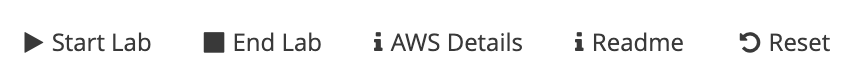
\includegraphics[width=\textwidth]{images/reset-button.png}

\noindent
To ensure that you are not accidentally depending on anything specific to your Learner Lab environment, we recommend that you reset your lab prior to final submission. Note that resetting the lab can take a considerable amount of time, in the order of hours. You should do this at \textit{least} 4 to 6 hours before the submission deadline. Please do not wait to the last minute.

\paragraph{Deploying with Docker}
In this course, you have been shown how to use Docker containers to deploy on ECS. You may refer to the practical worksheets for a description of how to deploy with containers \cite{prac-week5}.

\subsection{Fine Print}
You can reproduce our process for deploying your application using our \link{Docker image}{https://ghcr.io/CSSE6400/csse6400-cloud-testing}.
\codefile[language=docker]{Dockerfile}{deployment/Dockerfile}

Our steps for deploying your infrastructure using this container are as follows.
\texttt{\$REPO} is the name of your repository, and
\texttt{\$CREDENTIALS} is the path where we will store your AWS credentials.
\begin{code}[language=shell]{}
$ git clone git@github.com:CSSE6400/$REPO
$ cp $CREDENTIALS $REPO
$ docker run -v /var/run/docker.sock:/var/run/docker.sock -v $(pwd)/$REPO:/workspace csse6400-cloud-testing
$ cat $REPO/api.txt # this will be used for load-testing
\end{code}

Note that the Docker socket of the host has been mounted. This enables running \texttt{docker} in the container. This has been tested on Mac OSX and Linux but may require WSL2 on Windows.


\section{Criteria}
Your assignment submission will be assessed on its ability to support the specified use cases.
Testing is divided into functionality, deployment and scalability testing, corresponding to the three submission stages of the assignment.
Functionality testing is to ensure that your backend software and API meet the MVP requirements by satisfying the API specification without any excessive load.
Deployment is to ensure that this MVP can then be hosted in the target cloud provider.
Quality testing is based upon several likely use case scenarios.
The scenarios create different scaling requirements.

\subsection{API Functionality} % Pesistence: Does not need to be "truly" persistent.
40\% of the total marks for the assignment are for correctly implementing the API specification, irrespective of whether it is able to cope with high loads. A suite of automated API tests will assess the correctness of your implementation, via a sequence of API calls.

\subsection{Deployed to Cloud} % Persistence working correctly in the cloud.
25\% of the total marks for the assignment are for deploying a correctly implemented service to AWS irrespective of whether it is able to cope with high loads.
The deployment will be assessed by running a script that deploys your service to AWS and then runs a suite of automated API tests to assess the correctness of your implementation.

\subsection{Scalable Application}\label{sec:scenarios} % Can it scale!
The remaining 35\% of the marks will be derived from how well your service handles various scenarios.
These scenarios will require you to consider how your application performs under load.
Examples of possible scenarios are described below.
These are not descriptions of specific tests that will be run, rather they are examples of the types of tests that will be run.

\paragraph{Steady Stream}
Steady receipt of email messages at a rate of \emph{M} per minute, fairly evenly spread across all customers.
Approximately 20\% of the messages are malicious.

\paragraph{Bad `News' Stream}
Steady receipt of email messages at a rate of \emph{N} per minute, fairly evenly spread across all customers.
Approximately 80\% of the messages are malicious.

\paragraph{Peaks and Troughs}
Periods of receipt of a high volume of email messages, followed by periods of low volume.

\paragraph{High Value Customer}
The Department of Defence (DoD) has adopted SpamOverflow.
They are a high value customer and you must ensure that their requests are handled quickly.
All other customers have a service level agreement (SLA) that guarantees a certain level of responsiveness.
You cannot ignore their requests to only prioritise the DoD's requests.

\paragraph{Leaked Directory}
A bad actor has managed to get the email addresses of all employees of <Large Company>.
They have sent a phishing email to all of the users advertising a pay raise with a link to a fake login page.
The email is sent to all 10,000 employees at the same time.

\paragraph{Personalised Attack}
A bad actor has trained an AI model using social media profiles of targeted victims.
They can generate personalised phishing email messages based on personal information.
As the messages are personalised, they can be of greatly different lengths and contain different content.
These messages can only be identified by SpamHammer.
They have sent these phishing messages to 2,000 users at the same time.

\subsection{Marking}
Persistence is a core functional requirement of the system. If your implementation does not save email scans to persistent storage, your grade for the assignment will be capped at 4.

Your persistence mechanism must be robust, so that it can cope with catastrophic failure of the system. If all running instances of your services are terminated, the system must be able to restart and guarantee that it has not lost any data about emails for which it returned a success response to the caller. There will not be a test that explicitly kills all services and restarts the system. This will be assessed based on the services you use and how your implementation invokes those services. Not saving data to a persistent data store, or returning a success response before the data has been saved, are the criteria that determine whether you have successfully implemented persistence.

Functionality of your service is worth 40\% of the marks for the assignment. This is based on the successful implementation of the API specification given and the ability to use the given tool in your implementation.

Deploying your service is worth 25\% of the marks for the assignment. This is based on the successful deployment, using Terraform, of your service to AWS and the ability to access the service via the API. Your service must be fully functional while deployed so the functionality tests can be run which determines the marks for deployment.

Scaling your application to successfully handle the usage scenarios accounts for the other 35\% of the marks. The scenarios described in section \ref{sec:scenarios} provide guidance as to the type of scalability issues your system is expected to handle. They are not literal descriptions of the exact loads that will be used. Tests related to scenarios that involve more complex behaviour will have higher weight than other tests.

The scenarios will evaluate whether your service is being wasteful in resource usage. The amount of resources deployed in your AWS account will be monitored to ensure that your service implements a scaling up \emph{and} scaling down procedure.

All stages of the assessment will be marked using automation and a subset of the tests will be released. These tests may consume a \textbf{\emph{significant}} portion of your AWS credit. You are advised to be prudent in how many times you execute these tests. The amount of tests to be released is at the Course Coordinator's discretion.

Please refer to the marking criteria at the end of this document.

\subsubsection{Grade Improvement}\label{sec:improve}
Improving your application's functionality in a later submission will be used to improve the grade you received for an earlier submission.

\paragraph{Stage 1 Improvement}
If your stage 1 submission (API Functionality) performs poorly, you may improve your grade for this stage in a later stage.
This will occur if your deployed stage 2 or 3 submission passes more of the functionality tests than your stage 1 submission.
This new result will be used to recalculate your grade for stage 1.
(We will \textbf{not} rerun the local functionality tests in stages 2 or 3. We will \textbf{only} test your deployed application.)

\paragraph{Stage 2 Improvement}
Similarly, if your deployed stage 3 submission passes more of the functionality tests than your stage 2 submission, this result will be used to recalculate your grade for stage 2.

\paragraph{Late Penalties}
If an earlier submission was late, the same late penalty will be applied to your improved grade.
(e.g. If your stage 1 submission was 3 hours late, and in stage 2 your submission's functionality improved from a grade of 4 to a grade of 6,
your grade for stage 1 would be increased to a 5 after the one grade point per 24 hours penalty was applied.)

\section{Academic Integrity}
As this is a higher-level course, you are expected to be familiar with the importance of academic integrity in general, and the details of UQ's rules.
If you need a reminder, review the \link{Academic Integrity Modules} {https://web.library.uq.edu.au/library-services/it/learnuq-blackboard-help/academic-integrity-modules}.
Submissions will be checked to ensure that the work submitted is not plagiarised or of no academic merit.

This is an \textit{individual} assignment. You may \textbf{not} discuss details of approaches to solve the problem with other students in the course.
The Grade Improvement rule (section \ref{sec:improve}) means that you may \textbf{not} discuss details of any earlier submission stage with other students
until \textbf{two weeks} \textit{after} the final submission date of May 3$^{rd}$ (i.e. \textbf{May 20$^{th}$}).

All code that you submit \textbf{must} be your own work. You may \textbf{not} directly copy code that you have found on-line to solve parts of the assignment. If you find ideas from on-line sources (e.g. Stack Overflow), you must \link{cite and reference}{https://web.library.uq.edu.au/node/4221/2} these sources. Use the \link{IEEE referencing style}{https://libraryguides.vu.edu.au/ieeereferencing/gettingstarted} for citations and references. Citations should be included in a comment at the location where the idea is used in your code. All references for citations \textbf{must} be included in a file called \texttt{refs.txt}. This file must be in the top-level of your repository.

You may use generative AI tools (e.g. Copilot) to assist you in writing code to implement your solutions. You may also use generative AI tools to help you test your implementations. You \textbf{must} include, in the top-level of your repository, a file called \texttt{AI.md} that indicates the generative AI tools that you used, how you used them, and the extent of their use. (e.g. All code was written by providing copilot with class descriptions and then revising the generated code.)

Uncited or unreferenced material, or unacknowledged use of generative AI tools, will be treated as not being your own work. Significant amounts of cited or acknowledged work from other sources will be considered to be of no academic merit.

\bibliographystyle{ieeetr}
\bibliography{ours}

\clearpage

\newgeometry{left=12mm,right=7mm,top=5mm,bottom=12mm}

\begin{landscape}

\fontsize{9}{11}\selectfont

\begin{xltabular}{\linewidth}{| P{1.55cm} | X | X | X | X | X | X | X |}
\hline
\multicolumn{1}{|c}{\multirow{2}{*}{\textbf{Criteria}}} &
  \multicolumn{7}{c|}{\textbf{Standard}} \\ \cline{2-8} 
\multicolumn{1}{|c}{} &
  \multicolumn{1}{c|}{\textbf{Exceptional ~ (7)}} &
  \multicolumn{1}{c|}{\textbf{Advanced ~ (6)}} &
  \multicolumn{1}{c|}{\textbf{Proficient ~ (5)}} &
  \multicolumn{1}{c|}{\textbf{Functional ~ (4)}} &
  \multicolumn{1}{c|}{\textbf{Developing ~ (3)}} &
  \multicolumn{1}{c|}{\textbf{Little Evidence ~ (2)}} &
  \multicolumn{1}{c|}{\textbf{No Evidence ~ (1)}} \\ \hline
\endhead
%
\textbf{System\newline Scope\newline20\%} &
MVP's originally proposed functional \& non-functional requirements, or those agreed \& documented early in the project, are fully delivered. &
MVP's originally proposed functional \& non-functional~require\-ments, or those agreed \& documented early in the project, are delivered with small variances. &
MVP's functional \& non-functional requirements were revised \& documented later in the project, and are almost fully delivered. &
All important functional \& non-functional requirements are delivered but some other requirements are not, whether or not original plan was revised. &
Most important functional \& non-functional requirements are delivered, whether or not original plan was revised. &
Some important functional \& non-functional requirements are delivered, whether or not original plan was revised. &
Few important functional \& non-functional requirements are delivered, whether or not original plan was revised. \\
\hline

\textbf{Architecture\newline Suitability\newline 15\%} &
Delivered architecture, supplemented by the design reflection, is very well suited to delivering all specified functional \& non-functional require\-ments, including an appropriate level of security. &
Delivered architecture, supplemented by the design reflection, is~well suited to delivering~al\-most all specified functional \& non-functional requirements, including an appropriate level of security. &
Delivered architecture, supplemented by the design reflection, is fairly well suited to delivering the key functional \& non-functional requirements, including a mostly appropriate level of security. &
Delivered architecture, supplemented by the design reflection, is capable of delivering most key functional \& non-functional requirements, including a mostly appropriate level of security. &
Delivered architecture, supplemented by the design reflection, requires workarounds in a few cases to deliver key functional \& non-functional requirements. Design has one or two obvious security issues. &
Delivered architecture, supplemented by the design reflection, requires workarounds in several cases to deliver key functional \& non-functional requirements. Design has a few obvious security issues. &
Delivered architecture, supplemented by the design reflection, makes it difficult to deliver many functional \& non-functional requirements. Design does not appear to consider security issues. \\
\hline

\textbf{Testing\newline Quality\newline 20\%} &
All functional \& non-functional requirements, \& architectural components are well tested (or are described well in a test plan) and, where feasible, are automated. &
Most key functional \& non-functional require\-ments, \& key architec\-tural components are well tested (or are described adequately in a test plan) and, where feasible, are mostly automated. &
Most key functional \& non-functional require\-ments, \& key architec\-tural components are fairly well tested (or are described fairly adequately in a test plan) and, where feasible, many are automated. &
Most key functional \& non-functional require\-ments, \& key architectural components are fairly well tested (or are described fairly adequately in a test plan) and, with some attempt at automation. &
Main test cases for most key functional \& non-functional requirements, \& key architectural components are fairly well tested (or have some informative description in a test plan). &
Main test cases for a few key functional \& non-functional requirements, \& key architectural components are moderately well tested (or have a general description in a test plan). &
Testing is poor, superficial or extremely limited. Or, extent of testing cannot be determined from submitted artefacts. \\
\hline

\textbf{Architecture\newline Description\newline 25\%} &
Clear, accurate, concise \& complete description of all aspects of the architecture. Diagrams \& narrative text complement each other. Views enhance understanding all aspects of the architecture. Choice of architecture, \& decisions about design trade-offs, are well described. &
Clear, accurate \& mostly complete description of the architecture. Diagrams \& narrative text complement each other. Views support description of the architecture. Choice of architecture, \& decisions about important design trade-offs, are well described. &
Mostly clear, accurate \& complete description of the architecture. Diagrams \& narrative text support each other. Views support some description of the architecture. Choice of architecture, \& decisions about most important design trade-offs, are adequately described. &
Fairly clear, \& mostly accurate \& complete,~des- cription of the architecture. Diagrams \&~narra- tive text are consistent. Views provide little~sup- port describing the architecture.  Choice of~archi- tecture \& decisions about some important design trade-offs, are fairly adequately described. &
Some parts of the description are unclear, in- accurate or incomplete. Most diagrams are relevant to the narrative text or a necessary diagram is missing. Justification of choice of architecture is unclear. Decisions about a few important design trade-offs are fairly adequately described. &
Some parts of the description are inaccurate or incomplete, or many parts are unclear. Some diagrams are relevant to the narrative text or a few necessary diagrams are missing. Poor justification of choice of architecture. Few design trade-offs are adequately described. &
Many parts of the description are unclear, inaccurate or incomplete. Few diagrams are relevant to the narrative text or many necessary diagrams are missing. No, or very poor, justification of choice of architecture. Trade-offs are poorly described. \\
\hline

\textbf{Architecture\newline Evaluation\newline 20\%} &
Critique \& evaluation clearly demonstrate that the delivered architecture, varied a little by the reflection comments, can deliver all functional \& non-functional requirements of the full system. &
Critique \& evaluation clearly demonstrate~that the delivered architecture, varied by the reflection comments, can deliver all functional \& non-functional requirements of the full system. &
Critique \& evaluation demonstrate that the delivered architecture, varied by the reflection comments, can deliver all important functional \& non-functional requirements of the full system. &
Critique \& evaluation demonstrate that the delivered architecture, varied by the reflection comments, can deliver all important functional \& non-functional requirements of the MVP \& part of the full system. &
Critique \& evaluation demonstrate that the delivered architecture, varied by the reflection comments, can deliver all important functional \& non-functional requirements of the MVP but little of the full system. &
Critique \& evaluation demonstrate that the delivered architecture, varied by the reflection comments, can deliver some important functional \& non-functional requirements of the MVP. &
Critique \& evaluation demonstrate that the delivered architecture, varied by the reflection comments, is unlikely to deliver most functional or non-functional requirements of the MVP. Or, they are too unclear to determine. \\
\hline

\end{xltabular}

\end{landscape}

\restoregeometry

\end{document}


